% Asset ID: FA22GeneratingFunctionsTikZ-001
% Unit: FA22 – Further A2 2 Applied Mathematics
% Topic code: FA22-GENFUNC
% Topic ID: FA22GeneratingFunctions
% Related lesson: FA22_generating_functions_lesson.md
% Related section: # 9. Visual Asset Integration
% Source: CCEA core generating functions concept
% Purpose: Show coefficient extraction from an ordinary generating function.
\documentclass[tikz,border=8pt]{standalone}
\usepackage{amsmath}
\usepackage{xcolor}
\usetikzlibrary{arrows.meta, positioning, calc, shapes.geometric}
\definecolor{Canvas}{HTML}{FAF9F6}\definecolor{Ivory}{HTML}{FFFFF0}\definecolor{Line}{HTML}{E5E5EA}\definecolor{Gold}{HTML}{C5A059}\definecolor{SoftPink}{HTML}{FBEFEF}\definecolor{Text}{HTML}{2C2C2E}
\begin{document}
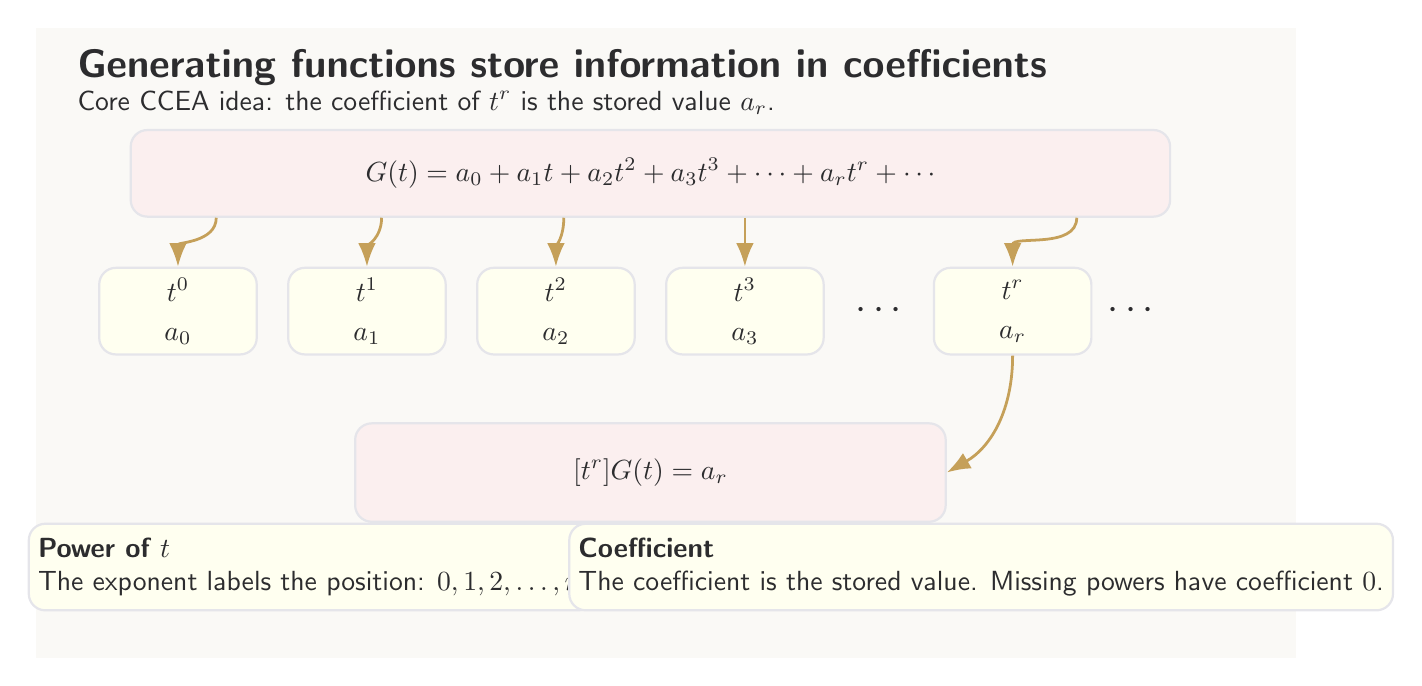
\begin{tikzpicture}[font=\sffamily,text=Text,box/.style={draw=Line,fill=Ivory,rounded corners=6pt,line width=0.8pt,minimum height=1.1cm,align=center},accentbox/.style={draw=Line,fill=SoftPink,rounded corners=6pt,line width=0.8pt,minimum height=1.1cm,align=center},arrow/.style={-{Latex[length=3mm]},line width=1pt,draw=Gold}]
\fill[Canvas] (-0.8,-2.8) rectangle (15.2,5.2);
\node[anchor=west,font=\sffamily\bfseries\Large] at (-0.4,4.7){Generating functions store information in coefficients};
\node[anchor=west,font=\sffamily\normalsize] at (-0.4,4.25){Core CCEA idea: the coefficient of \(t^r\) is the stored value \(a_r\).};
\node[accentbox,minimum width=13.2cm] (gf) at (7,3.35){\(\displaystyle G(t)=a_0+a_1t+a_2t^2+a_3t^3+\cdots+a_rt^r+\cdots\)};
\node[box,minimum width=2.0cm] (d0) at (1,1.6){\(\displaystyle t^0\)\\[2pt]\(\displaystyle a_0\)};
\node[box,minimum width=2.0cm] (d1) at (3.4,1.6){\(\displaystyle t^1\)\\[2pt]\(\displaystyle a_1\)};
\node[box,minimum width=2.0cm] (d2) at (5.8,1.6){\(\displaystyle t^2\)\\[2pt]\(\displaystyle a_2\)};
\node[box,minimum width=2.0cm] (d3) at (8.2,1.6){\(\displaystyle t^3\)\\[2pt]\(\displaystyle a_3\)};
\node[box,minimum width=2.0cm] (dr) at (11.6,1.6){\(\displaystyle t^r\)\\[2pt]\(\displaystyle a_r\)};
\node[font=\Large] at (9.9,1.6){\(\cdots\)};\node[font=\Large] at (13.1,1.6){\(\cdots\)};
\draw[arrow] (gf.south west) ++(1.1,0) to[out=-90,in=90] (d0.north);\draw[arrow] (gf.south west) ++(3.2,0) to[out=-90,in=90] (d1.north);\draw[arrow] (gf.south) ++(-1.1,0) to[out=-90,in=90] (d2.north);\draw[arrow] (gf.south) ++(1.2,0) to[out=-90,in=90] (d3.north);\draw[arrow] (gf.south east) ++(-1.2,0) to[out=-90,in=90] (dr.north);
\node[accentbox,minimum width=7.5cm,minimum height=1.25cm] (extract) at (7,-0.45){\(\displaystyle [t^r]G(t)=a_r\)};
\draw[arrow] (dr.south) to[out=-90,in=30] (extract.east);
\node[box,minimum width=5.4cm,align=left] at (2.7,-1.65){\textbf{Power of \(t\)}\\The exponent labels the position: \(0,1,2,\ldots,r\).};
\node[box,minimum width=5.4cm,align=left] at (11.2,-1.65){\textbf{Coefficient}\\The coefficient is the stored value. Missing powers have coefficient \(0\).};
\end{tikzpicture}
\end{document}
